\section{Results}
The hypotheses about social and linguistic dissemination are tested under four analyses: correlation against frequency change in growth words; causal inference on probability of word growth; binary prediction of word growth; and survival analysis of decline words.
%We find evidence in support of hypotheses H1, H2 and H2a, such that both social dissemination and context dissemination play an important role in predicting innovation success.

\subsection{Correlational analysis}
\label{subsec:relative-importance}
To test the relative importance of the linguistic and social context on word growth, we correlate these metrics with frequency change ($\Delta_{f_{t}} = f_{t} - f_{t-k}$) across all growth words. 
This replicates the methodology in prior work by \newcite{altmann2011} and \newcite{garley2012}, who analyzed different internet forums.
Focusing on long-term change with $k=12$ (one year) and $k=24$ (two years), 
%we compute the correlation between each covariate at time $t-k$ and the frequency change from $t-k$ to $t$,
we compute the proportion of variance in frequency change explained by the covariates using a relative importance regression~\cite{kruskal1987}.\footnote{Relative importance regression implemented in the \emph{relaimpo} package in R: \url{https://cran.r-project.org/package=relaimpo}}

The results of the regression are shown in \autoref{tab:relative-importance-test}. 
All predictors have relative importance greater than zero, according to a bootstrap method to produce confidence intervals~\cite{tonidandel2009}. 
Frequency is the strongest predictor ($f_{t-12}, f_{t-24}$), because words with low initial frequency often show the most frequency change.
In both short- and long-term prediction, linguistic dissemination ($D^{L}_{t-12}, D^{L}_{t-24}$) has a higher relative importance than each of the social dissemination metrics.
%, indicating the importance of lexical flexibility in predicting word growth. 
The social dissemination metrics have less explanatory power, in comparison with the other predictors and in comparison to the prior results of \newcite{garley2012}, who found $1.5\%$ of variance explained by $D^{U}$ and $1.9\%$ for $D^{T}$ at $k=24$.
Our results were robust to the exclusion of the predictor $D^L$, meaning that a model with only the social dissemination metrics as predictors resulted in a similar proportion of variance explained.
The weakness of social dissemination could be due to the fragmented nature of Reddit, compared to more intra-connected forums. 
Since users and threads are spread across many different subreddits, and users may not visit multiple subreddits, a higher social dissemination for a particular word may not lead to immediate growth.

\begin{table}[t!]
\small
\centering
\begin{tabular}{l r r }
  \toprule
  ~ & \specialcell{Variance \\ explained} & Lower, upper 95\% \\
  \midrule
$f_{t-12}$ & 10.8\% & [10.2\%, 11.5\%]  \\ 
$D^{L}_{t-12}$ & 0.584\% & [0.461\%, 0.777\%]  \\ 
$D^{U}_{t-12}$ & 0.307\% & [0.251\%, 0.398\%] \\ 
$D^{S}_{t-12}$ & 0.120\% & [0.0852\%, 0.191\%] \\ 
$D^{T}_{t-12}$ & 0.246\% & [0.171\%, 0.379\%]  \\[2ex]
$f_{t-24}$ & 21.4\% & [20.4\%, 22.4\%] \\ 
$D^{L}_{t-24}$ & 1.29\% & [1.05\%, 1.64\%] \\ 
$D^{U}_{t-24}$ & 0.400\% & [0.346\%, 0.493\%] \\ 
$D^{S}_{t-24}$ & 0.287\%  & [0.201\%, 0.392\%] \\ 
$D^{T}_{t-24}$ & 0.272\% & [0.226\%, 0.380\%] \\ \bottomrule
% output/results/relative_importance_coefficients_f_DU_DS_DT_DL.tsv
\end{tabular}

\caption{Percent of variance explained in frequency change, computed over all growth words $\set{G}$.
$N=26,880$ for $k=12$, $N=13,440$ for $k=24$.} 
\label{tab:relative-importance-test}
\end{table}

\subsection{Causal analysis}
\label{sec:results-causal}
While correlation can help explain the relationship between dissemination and frequency change, it only addresses the weak version of H2: it does not distinguish the causal impact of linguistic and social dissemination. 
To test the strong version of H2, we turn to a causal analysis, in which the \emph{outcome} is whether a nonstandard word grows or declines, the \emph{treatment} is a single dissemination metric such as linguistic dissemination, and the \emph{covariates} are the remaining dissemination metrics. 
The goal of this analysis is to test the impact of each dissemination metric, while holding the others constant. 

\begin{figure*}
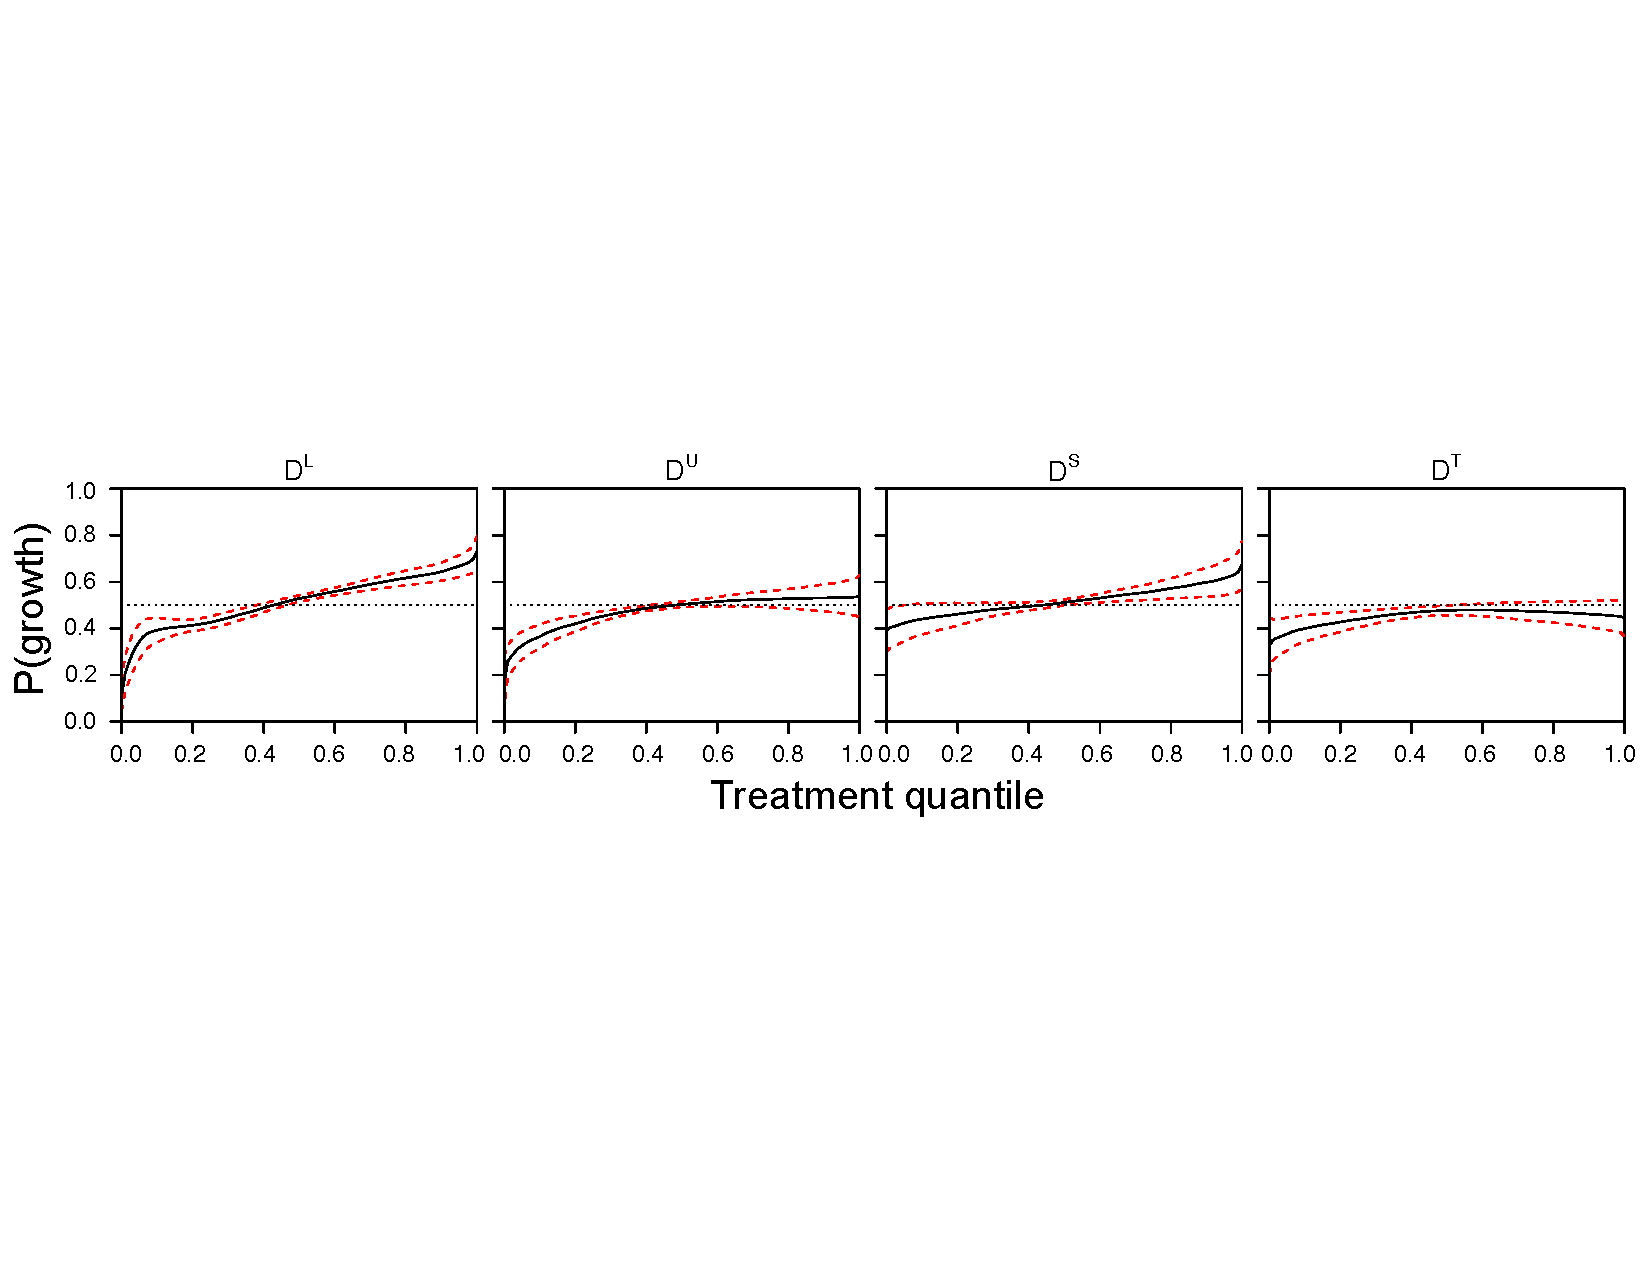
\includegraphics[width=\textwidth]{figures/ADRF_curves_1_12_100_DL,DU,DS,DT.pdf}
% generated with scripts/prediction/plot_average_dose_response_function.R
\caption{Average dose response function for all treatment variables, where outcome is probability of word growth. 95\% confidence intervals plotted in red, chance rate of 50\% marked with dotted black line.}
\label{fig:ADRF_curves}
\end{figure*}

Causal inference typically uses a binary treatment/control distinction~\cite{angrist1996}, but in this case the treatment is continuous. 
We therefore turn to an adapted model known as the \emph{average dose response function} to measure the causal impact of dissemination~\cite{imbens2000}.
To explain the procedure for estimating the average dose response, we adopt the following terminology: $Z$ for treatment variable, $X$ for covariates, $Y$ for outcome.\footnote{Average dose response function implemented in the \emph{causaldrf} package in R: \url{https://cran.r-project.org/package=causaldrf}}
\begin{enumerate}
\setlength{\itemsep}{1pt}
\item A linear model is fit to estimate the treatment from the covariates,
  \begin{equation}
    Z_{i} \mid X_{i} \sim \mathcal{N}(\beta^{\top} X_{i},\sigma^{2}).
  \end{equation}
  The output of this estimation procedure is a vector of weights $\hat{\beta}$ and a variance $\hat{\sigma}^2$. 
\item The generalized propensity score (GPS) $R$ is the likelihood of observing the treatment given the covariates, $P(Z_{i} \mid X_{i})$. It is computed from the parameters estimated in the previous step:
  \begin{equation}
    \hat{R}_i = \frac{1}{\sqrt{2\pi\hat{\sigma}^{2}}} \exp \left(-\frac{(Z_{i} - \hat{\beta}^{\top}X_{i})^{2}}{2\hat{\sigma}^{2}}\right).
  \end{equation}
\item A logistic model is fit to predict the outcome $Y_{i}$ using the treatment $Z_{i}$ and the GPS $\hat{R}_i$:
  \begin{equation}
    \hat{Y}_{i} = \text{Logistic}(\hat{\alpha}_{0} + \hat{\alpha}_{1}Z_{i} + \hat{\alpha}_{2}\hat{R}_i).
  \end{equation}
  This involves estimating the parameters $\{\hat{\alpha}_0, \hat{\alpha}_1, \hat{\alpha}_2.\}$
By incorporating the generalized propensity score $\hat{R}_i$ into this predictive model over the outcome, it is possible to isolate the causal effect of the treatment from the other covariates~\citep{hirano2004}.
\item The range of treatments is divided into levels (quantiles). The \emph{average dose response} for a given treatment level $s_{z}$ is the mean estimated outcome for all instances at that treatment level,
\begin{equation}
\hat{\mu}(s_{z}) = \frac{1}{| s_{z} |} \sum_{z_{i} \in s_{z}} \hat{Y}_{i}.
\end{equation}
The average dose response function is then plotted for all treatment levels.
\end{enumerate}

Each dissemination metric is considered separately as a treatment. 
We consider all other dissemination metrics and frequency as covariates: e.g., for treatment variable $D^{L}$, the covariates are set to $[f,D^{U},D^{S},D^{T}]$.
We bootstrap the above process 100 times with different samples to produce confidence intervals.
To balance the outcome classes, we sample an equal number of growth and decline words for each bootstrap iteration.

The average dose response function curves in \autoref{fig:ADRF_curves} show that linguistic dissemination ($D^{L}$) produces the most dramatic increase in word growth probability.
For linguistic dissemination, the lowest treatment quantile (0\%-10\%) yields a growth probability below 40\% (significantly less than chance), as compared to the highest treatment quantile (90-100\%), which yields a growth probability nearly at 70\% (significantly greater than chance). 
This supports the strong form of H2, which states that linguistic dissemination is predictive of growth, even after controlling for the frequency and the other dissemination metrics. 
Subreddit dissemination also shows a mild causal effect on word growth, up to 60\% in the highest treatment quantile.
The other social dissemination metrics prove to have less effect on word growth.

\subsection{Predictive analysis}
\label{sec:results-binary-predict}
We now turn to prediction to determine the utility of linguistic and social dissemination: using the first $k$ months of data, can we predict whether a word will grow or decline in popularity?
This is similar to previous work in predicting the success of lexical innovations~\cite{kooti2012predicting}, but our goal is to compare the relative predictive power of various dissemination metrics, rather than to maximize accuracy.

\begin{figure}
\centering
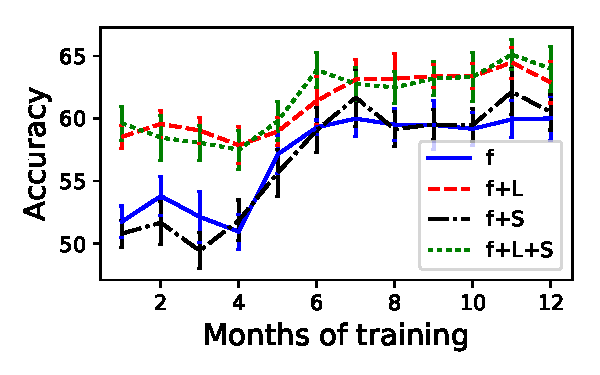
\includegraphics[width=\columnwidth]{figures/success_1_12_window_lines.pdf}
\caption{Prediction accuracy for different feature sets using $k={1...12}$ months of training data. $f$ indicates frequency-only, $f+L$ frequency plus linguistic dissemination, $f+S$ frequency plus social dissemination, $f+L+S$ all features.}
\label{fig:success_accuracy}
% scripts/prediction/plot_growth_k_month_window_lines.py
\end{figure}

We use logistic regression with 10-fold cross-validation over four different feature sets: frequency-only (\model{f}), frequency plus linguistic dissemination (\model{f+L}), frequency plus social dissemination (\model{f+S}) and all features (\model{f+L+S}).
Each fold is balanced for classes so that the baseline accuracy is 50\%.
\autoref{fig:success_accuracy} shows that linguistic dissemination provides more predictive power than social dissemination: the accuracy is consistently higher for the models with linguistic dissemination than for the frequency-only and social dissemination models.
The accuracies converge as the training data size increases, which suggests that frequency is a useful predictor if provided sufficient historical trajectory.

%% ADRF prediction

%\begin{figure}[t!]
%\centering
%\includegraphics[width=0.7\columnwidth]{figures/ADRF_accuracy_1_12_DL,DS,DU,DT,f.pdf}
%% generated with scripts/prediction/plot_average_dose_response_function_accuracy.R
%\caption{Accuracy on predicting success from fail words using different treatment models (10-fold cross-validation).}
%\label{fig:ADRF_accuracy}
%\end{figure}

%We further investigate the predictive power of the different dissemination metrics as follows: using the parameters estimated for the dose response function, what is the accuracy of predicting lexical success?

%For each treatment variable, a logistic regression model is parameterized using the mean of the parameters computed in (3) and used to predict success versus failure using the first $k=12$ months of data.
%The baseline model is a frequency-only logistic regression in which the mean frequency over the first $k=12$ months of data is used to predict success versus failure.
%This process is conducted using 10-fold cross-validation and the AUC accuracy is measured to compare the predictive power of different treatments.
%The results in~\autoref{fig:ADRF_accuracy} demonstrate that the model using linguistic dissemination (DL) performs the best (66\%), followed by the model with user dissemination (DU; 60\%).
%This aligns with the results from the ADRF curves, which showed a significant difference in probability of success between the low- and high-treatment conditions.

\begin{figure}
\centering
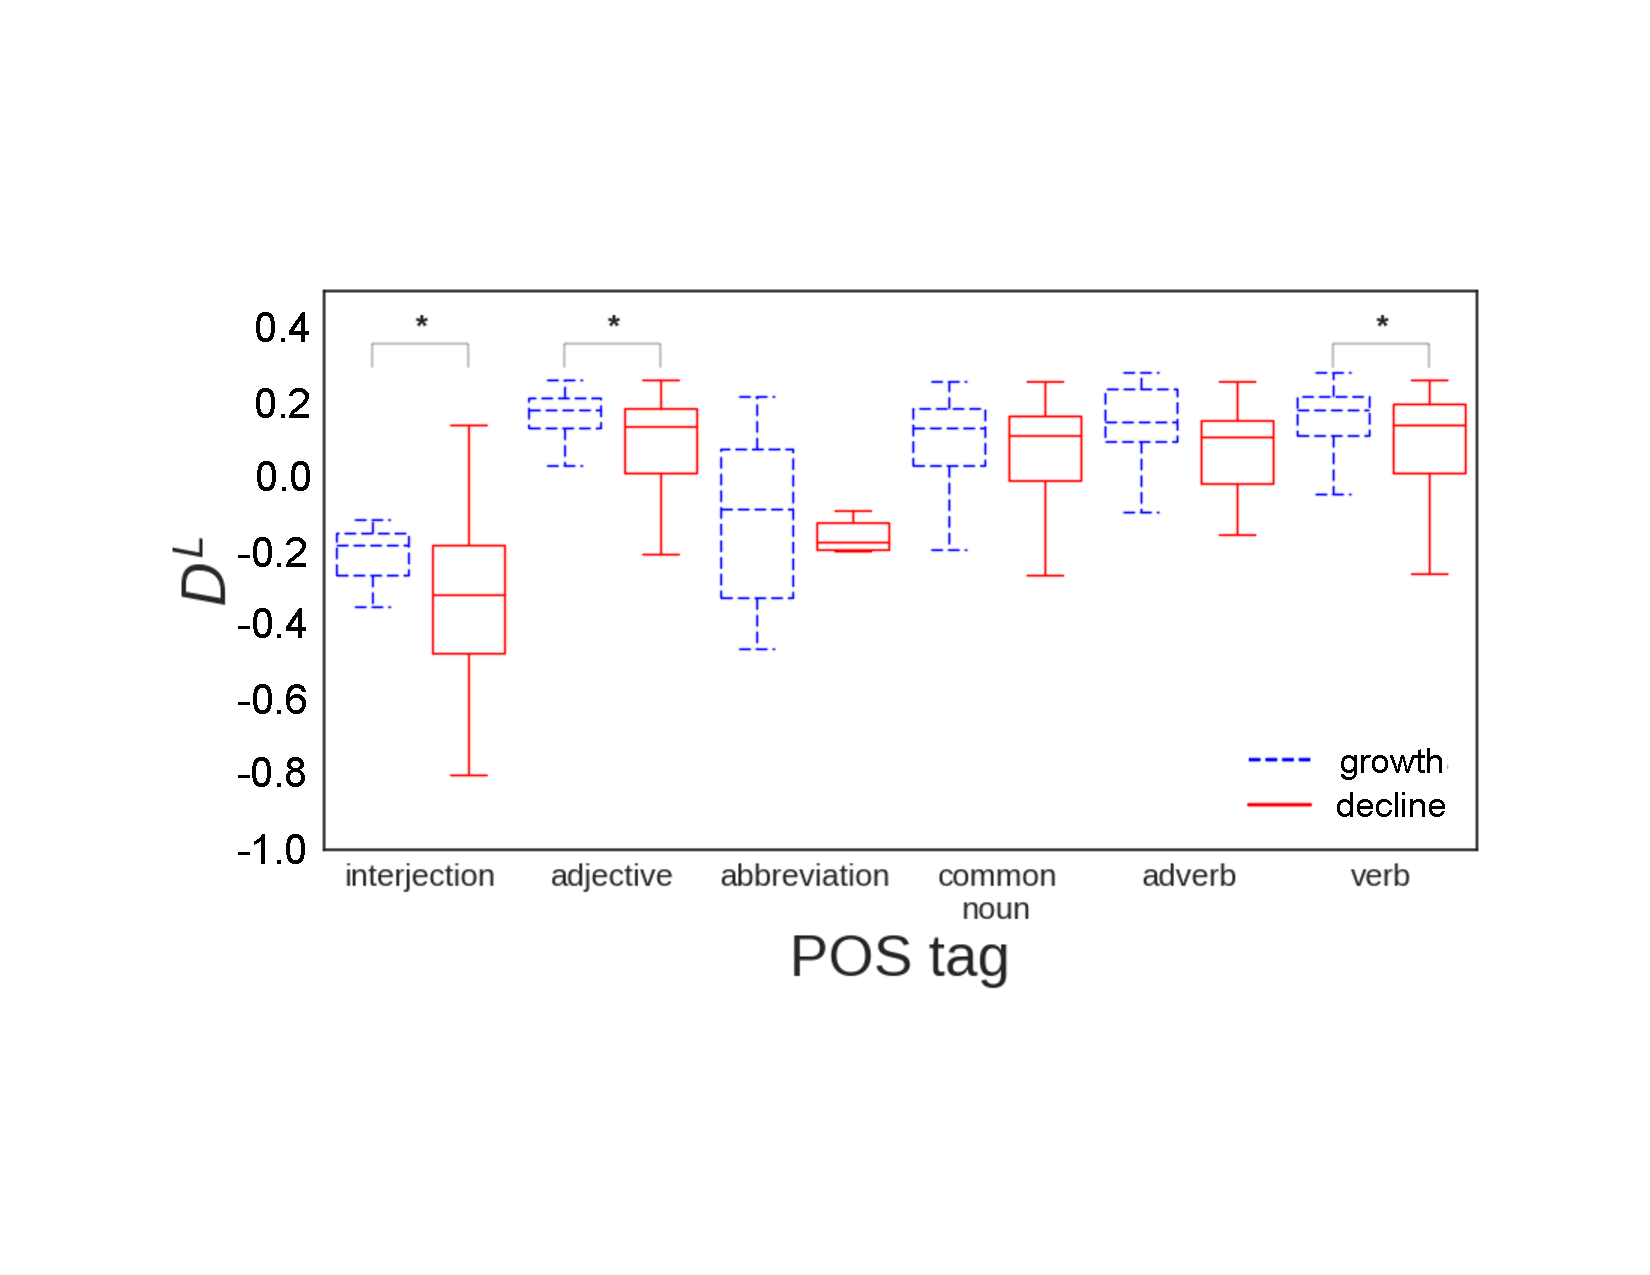
\includegraphics[width=\columnwidth]{figures/growth_vs_decline_matched_pos_DL_distribution_1_12.pdf}
% generated with scripts/frequency/plot_success_vs_failure_pos_DL_distribution.sh
\caption{Distribution of $D^{L}$ values across growth and decline words, grouped by part of speech tag. 
* indicates $p<0.05$ in one-tailed t-test between growth and decline $D^{L}$ values.}
\label{fig:success_vs_failure_pos_DL_distribution}
\end{figure}

\paragraph{Part-of-speech robustness check}

Considering the uneven distribution of linguistic dissemination across part-of-speech groups (\autoref{fig:pos-cd-dist}), the prediction results may be explained by an imbalance of word categories between the growth and decline words.
This issue is addressed through two robustness checks: within-group comparison and prediction.

First, we compare the distribution of linguistic dissemination values between growth and decline words, grouped by the most common POS tags (computed in \autoref{sec:linguistic_dissemination}).
Each decline word is matched with a growth word based on similar mean frequency in the first $k=12$ months, and their mean linguistic dissemination values during that time period are compared, grouped within POS tag groups.
The differences in~\autoref{fig:success_vs_failure_pos_DL_distribution} show that across all POS tags, the growth words show a tendency toward higher linguistic dissemination with significant ($p<0.05$) differences in the interjections and verbs.

%To address this possibility, the POS tags (computed in \autoref{sec:linguistic_dissemination}) are added as additional features to the binary prediction task.
Next, we add POS tags as additional features to the frequency-only model in the binary prediction task.
The accuracy of a predictive model with access to frequency and POS features at ${k=1}$ is 54.8\%, which is substantially lower than the accuracy of the model with frequency and linguistic dissemination (cf. \autoref{fig:success_accuracy}).\footnote{Higher $k$ values yield similar results.}
Thus, linguistic dissemination thus contributes predictive power beyond what is contributed by part-of-speech alone.
% scripts/prediction/predict_growth_POS_tag.py

\subsection{Survival analysis}
\label{sec:results-survival}
Having investigated what separates growth from decline, we now focus on the factors that precede a decline word's ``death'' phase~\cite{drouin2009}.
%We now focus on the factors that precede a word's decline phase, which can be viewed as the beginning of ``word death''~\cite{drouin2009} for many of these terms --- though some may emerge again later. 
%We use the decline words as ``uncensored'' data, words with an observed death date, and the growth words as ``censored'' data, words with an unobserved death date.
%The distribution of survivors is shown in Figure \ref{fig:split_point_dist}, which shows that most of the decline words begin to decline before the year mark ($t=12$). 
%\begin{figure}[t!]
%\centering
%\includegraphics[width=\columnwidth]{figures/split_point_survivor_curve.pdf}
%\caption{Survival curve of all decline and growth words.}
%%\caption{Survival curve of all failure and success innovations, dotted line indicates number of success (i.e. non-death) innovations.}
%\label{fig:split_point_dist}
%\end{figure}
Predicting the time until a word's decline can be framed as survival analysis~\cite{klein2005}, in which a word is said to ``survive'' until the beginning of its decline phase at split point $\hat{t}$. 
In the Cox proportional hazards model~\cite{david1972}, the hazard of death $\lambda$ at each time $t$ is modeled as a linear function of a vector of predictors,
\begin{equation}
  \lambda_i(t)  = \lambda_0(t) \exp (\mathbf{\beta} \cdot \mathbf{x}_i),
\end{equation}
where $\mathbf{x}_i$ is the vector of predictors for word $i$, and $\mathbf{\beta}$ is the vector of coefficients. Each cell $x_{i,j}$ is set to the mean value of predictor $j$ for word $i$ over the training period $t=\{1 ... k\}$ where $k=3$.

For words which begin to decline in popularity in our dataset, we treat the point of decline as the ``death'' date. The remaining words are viewed as \emph{censored} instances: they may begin to decline in popularity at some point in the future, but this time is outside our frame of observation.
We use frequency, social dissemination and linguistic dissemination as predictors in a Cox regression model.\footnote{Cox regression implemented in the \emph{lifelines} package in Python: \url{https://lifelines.readthedocs.io/en/latest/}.}

\begin{table}[t!]
\small
\centering
\begin{tabular}{l r r r r}
\toprule
  Predictor & $\beta$ & std. error & $Z$ & $p$ \\ \midrule
% old results
%$f$ & -0.208 & 0.0399 & -5.21 & *** \\ 
%$D^{L}$ & -0.310 & 0.0346 & -8.96 & *** \\ 
%$D^{U}$ & -0.0845 & 0.0583 & -1.45 & ~ \\ 
%$D^{S}$ & -0.127 & 0.0596 & -2.13 & * \\ 
%$D^{T}$ & 0.0819 & 0.0727 & 1.13 & ~ \\ 
$\var{f}$ & -0.207 & 0.0492 & -4.21 & *** \\ 
$\var{D^{L}}$ & -0.330 & 0.0385 & -8.56 & *** \\ 
$\var{D^{U}}$ & 0.0053 & 0.0518 & 0.102 & ~ \\ 
$\var{D^{S}}$ & -0.156 & 0.0807 & -1.928 & ~ \\ 
  $\var{D^{T}}$ & 0.0825 & 0.0662 & 1.25 & ~ \\
  \bottomrule
\end{tabular}
\caption{Cox regression results for predicting word death with all predictors (\model{f+L+S}) averaged over first $k=3$ months.
%Concordance=0.623, where 0.50 represents random chance. 
*** indicates $p<0.001$, otherwise $p>0.05$.}
%\ian{results with $t={0:3}$}}
\label{tab:cox_regression_growth_decline_up_to_3}
% prediction/survival_analysis_python.ipynb#Limited-time-range
% prediction/survival_analysis_tests.py
% output/cox_regression_first_3.txt
\end{table}

The estimated coefficients from the regression are shown in \autoref{tab:cox_regression_growth_decline_up_to_3}.
We find 
%a weak positive coefficient for bigram context diversity and 
a negative coefficient for linguistic dissemination ($\beta=-0.330, p<0.001$), which mirrors the results from \autoref{sec:results-causal}: 
%higher $C^{2}$ and 
higher $D^{L}$ indicates a lower hazard of word death, and therefore a higher likelihood of survival.
%We also find weak negative coefficients ($p>0.05$) for user and subreddit dissemination, suggesting 
We also find that higher subreddit dissemination has a weak but insignificant correlation with a lower likelihood of word death ($\beta=-0.156, p>0.05$).
Both of these results lend additional support to the strong form of the hypothesis H2.
%Thread dissemination pointed in the opposite direction 
%(consistent with the finding from ~\newcite{altmann2011}), (cf. Fig 4 in Altmann et al 2011)
%and user dissemination had no significant effect. 

%\begin{table}[t!]
%\small
%\centering
%\begin{tabular}{l l l l l}
  \toprule
Model & Deviance & d.f. & $\chi^{2}$ & $p$-value \\ \midrule
Null & 4383 & 0 & ~ & ~ \\ 
\model{f} & 4375 & 1 & 16.19 & *** \\ 
\model{f+S} & 4370 & 4 & 27.24 & *** \\ 
\model{f+L} & 4337 & 2 & 93.32 & *** \\ 
\model{f+L+S} & 4331 & 5 & 103.8 & *** \\ 
\bottomrule
%output/cox_regression_deviance_output.txt
\end{tabular}
%\caption{Deviance values for relevant survival models.
%%survival model that uses frequency ($f$), frequency plus dissemination ($f+S$), frequency plus context diversity ($f+L$), and frequency plus context diversity plus dissemination ($f+L+S$). 
%$\chi^{2}$ values based on the likelihood ratio test comparing each model to the null model. 
%Lower deviance indicates better model fit.
%*** indicates $p<0.001$.}
%\label{tab:cox_regression_deviance}
%%survival_analysis_R.ipynb#Survival-analysis-separate-factors
%\end{table}

%The role of each factor is tested by comparing the goodness-of-fit for Cox regression models using different feature sets: frequency (\model{f}), frequency plus linguistic dissemination (\model{f+L}), frequency plus social dissemination (\model{f+S}) and all factors (\model{f+L+S}). 
%The results in \autoref{tab:cox_regression_deviance} demonstrate that the model with dissemination and the model with linguistic diversity each have significantly better-than-null fits (lower deviance than null model).
%However, the all-factor model (\model{f+L+S}) does not have a significantly lower deviance than the linguistic dissemination model (\model{f+L}) ($\chi^{2}=4.6, p=0.80$), therefore adding social dissemination does not significantly improve the model fit. 
%This points to the especially important role of linguistic dissemination in predicting the word growth, as compared with social dissemination.

The predictive accuracy of survival analysis can be quantified by a \emph{concordance score}. A score of 1.0 on heldout data indicates that the model perfectly predicts the order of death times; a score of 0.5 indicates that the predictions are no better than a chance ordering. We perform 10-fold cross-validation of the survival analysis model, and plot the results in \autoref{fig:cox_regression_concordance_scores}.
%To compare the predictive performance of the separate Cox models, we compute their concordance scores using 10-fold cross-validation.\footnote{The concordance score represents the accuracy of predicting the order of death times: a score of 0.5 implies a random order of death times, and a score of 1.0 implies a perfect order of death times.}
%As shown in \autoref{fig:cox_regression_concordance_scores}, the model incorporating
The model with access to linguistic dissemination (\model{f+L}) consistently achieves higher concordance than the baseline frequency-only model (\model{f}), 
%according to Welch's t-test 
($t=4.29, p<0.001$), and the model with all predictors \model{f+L+S} significantly outperforms the model with access only to frequency and social dissemination \model{f+S} ($t=4.64, p<0.001$).
The result is reinforced by testing the goodness-of-fit for each model with model \emph{deviance}, or difference from the null model. 
The \model{f+L} model has lower deviance, i.e. better fit, than the null model ($\chi^{2}=93.3, p < 0.01$), and the \model{f+L+S} does not have a significantly lower deviance than the \model{f+L} model ($\chi^{2}=4.6, p=0.80$), suggesting that adding social dissemination does not significantly improve model fit.

% output/concordance_score_feature_set_comparison_tests.tsv
\begin{figure}[t!]
\centering
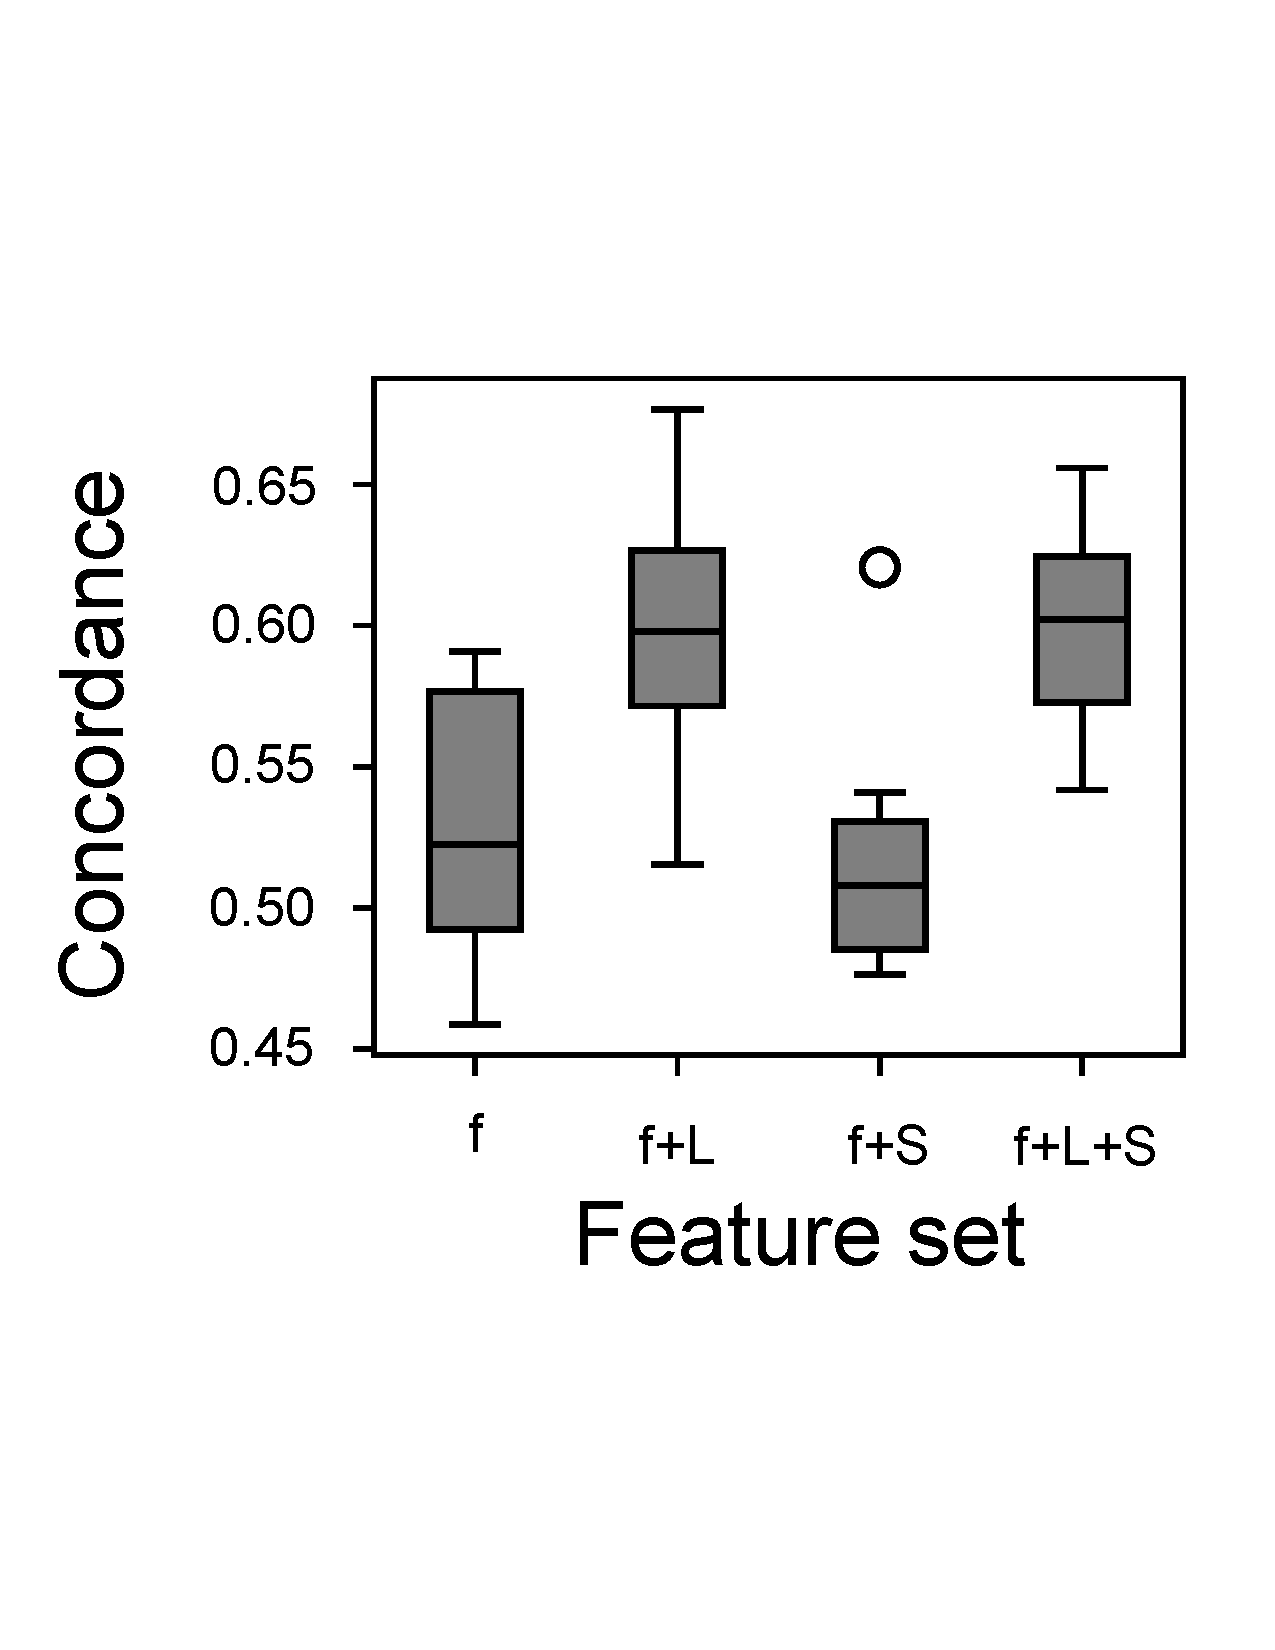
\includegraphics[width=0.8\columnwidth]{figures/survival_concordance_score_distribution.pdf}
\caption{Distribution of concordance scores (10-fold cross-validation) of the Cox regression models across feature sets.}
\label{fig:cox_regression_concordance_scores}
% prediction/plot_concordance_scores.py
\end{figure}



%%%%%%%%%%%%%%%%%%%%%%%%%%%% OLD STUFF

%We therefore test the relative predictive power of the different dissemination metrics with two tests: (1) causal inference and (2) binary prediction of success versus failure.

%\begin{figure}[t!]
%\centering
%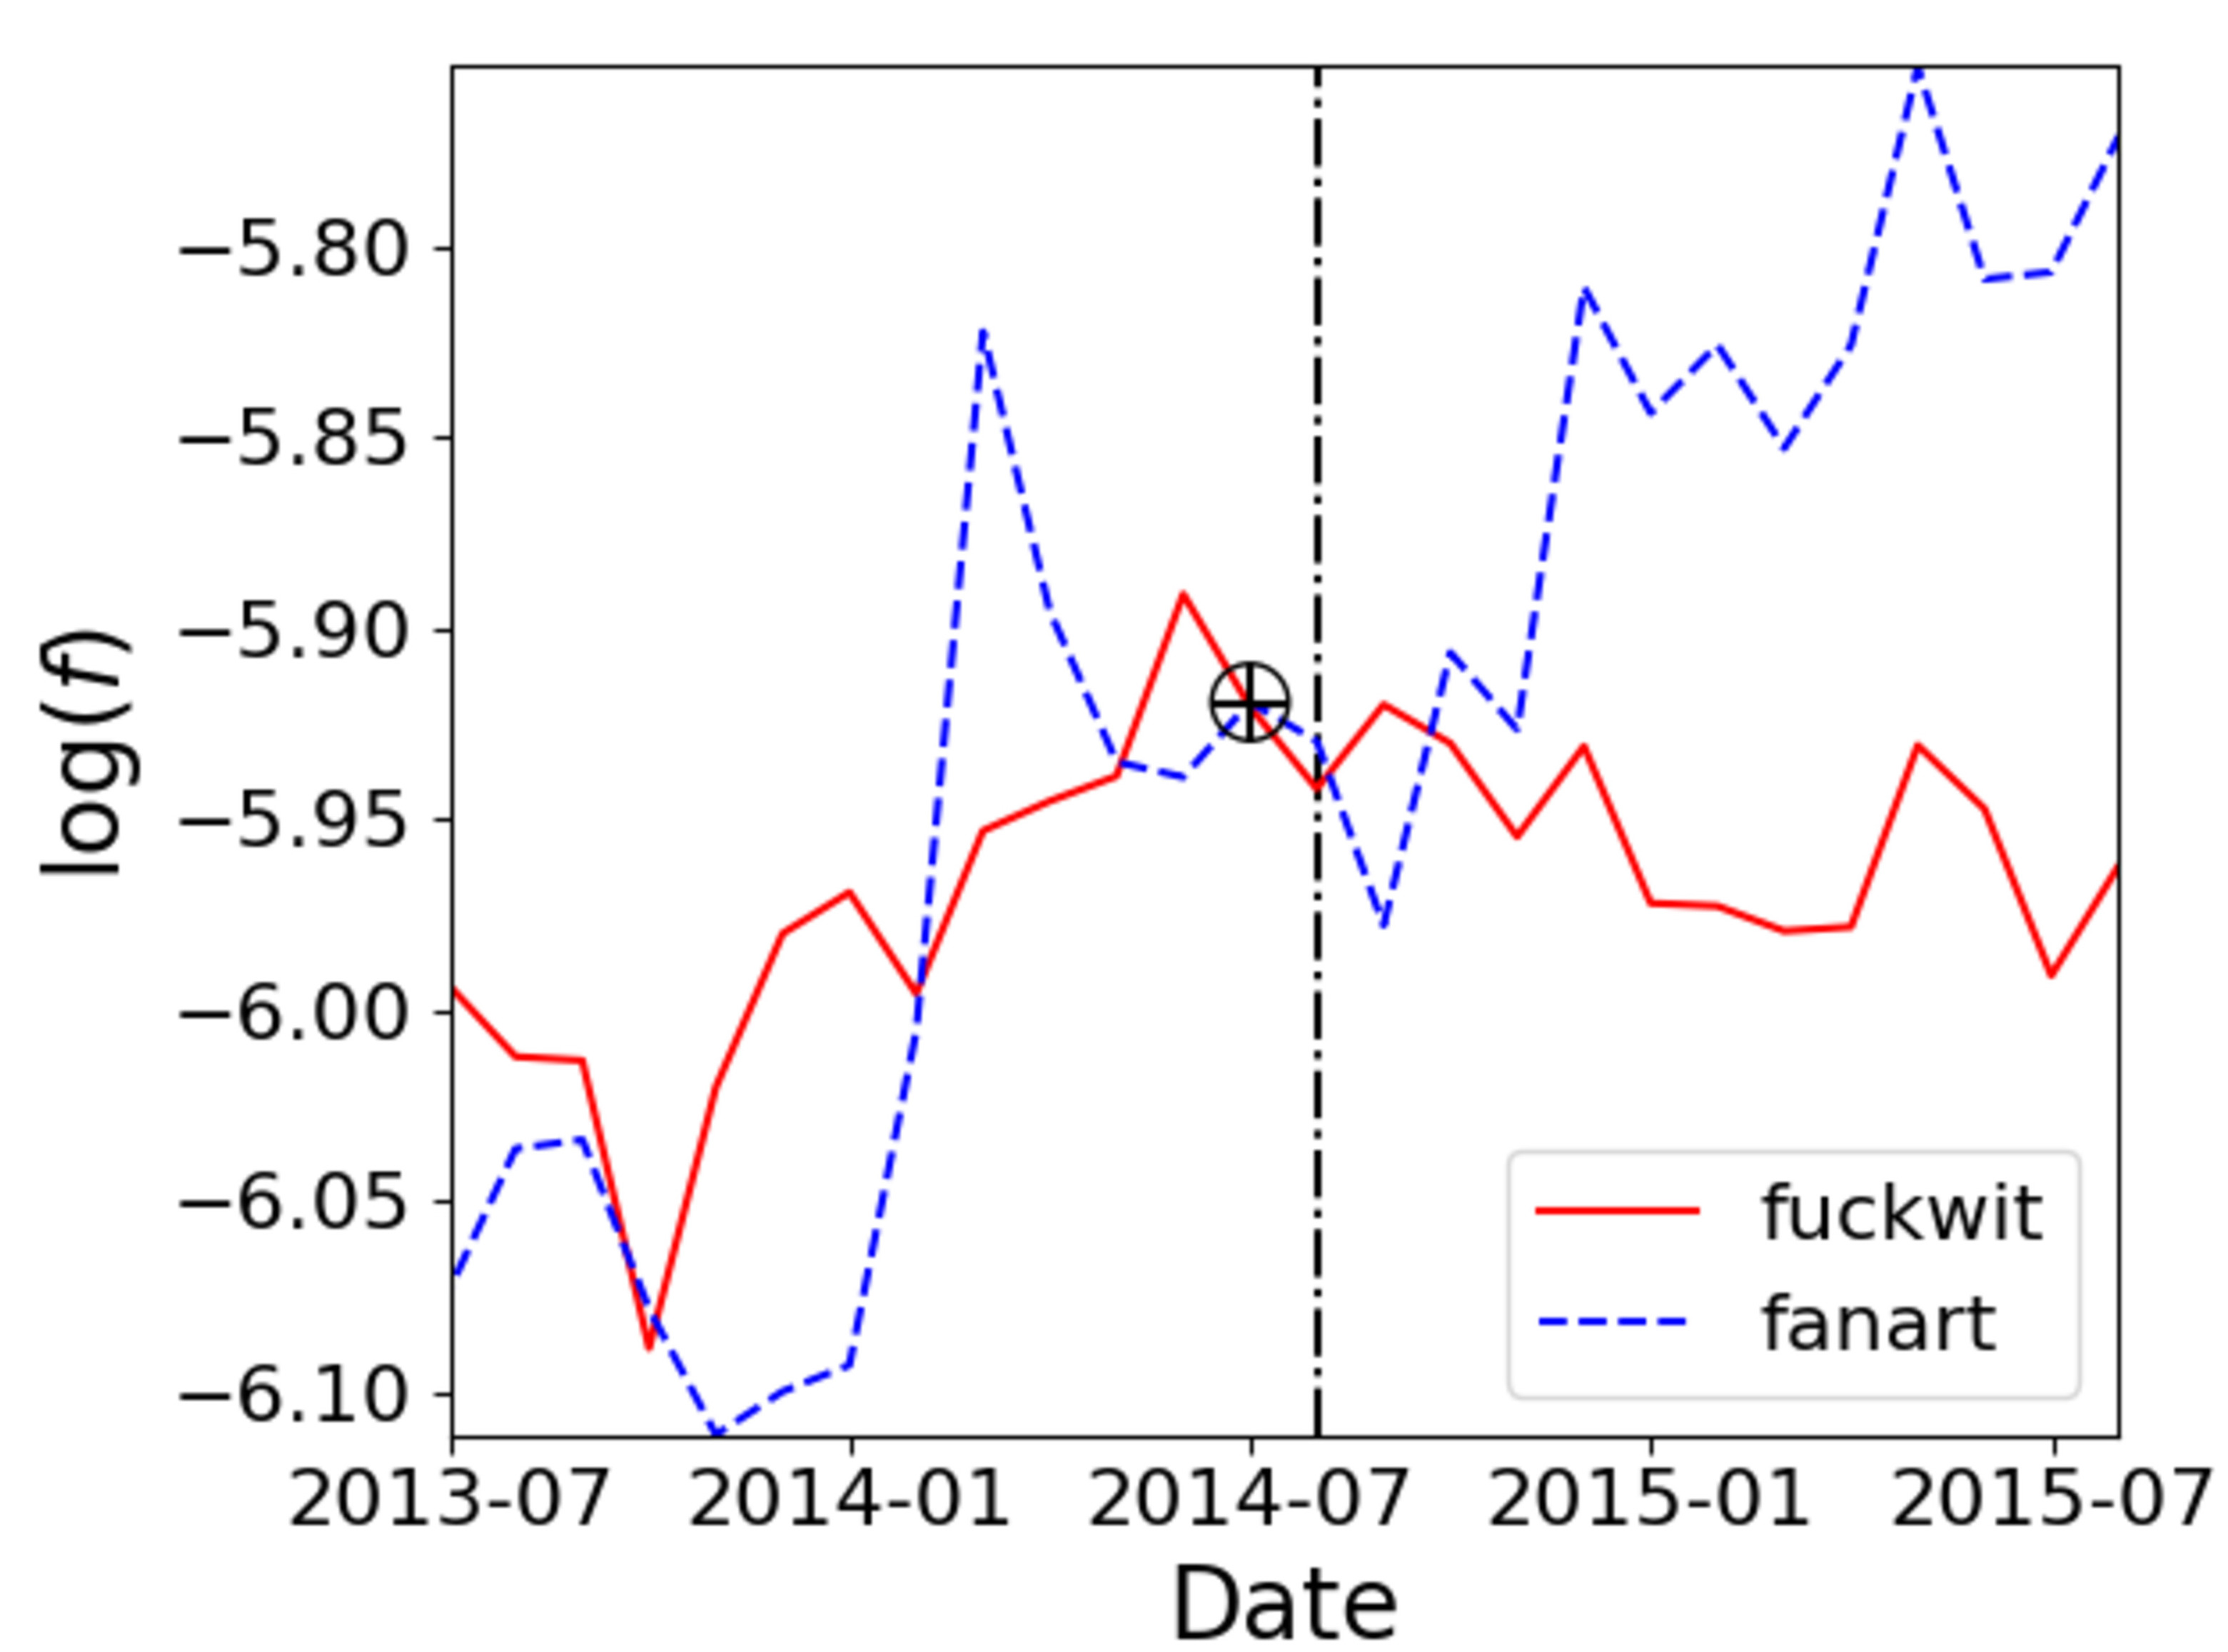
\includegraphics[width=1.0\columnwidth]{figures/match_time_series_example.png}
%\caption{Example failed innovation \example{fuckwit} (\gloss{idiot}) with matched successful innovation \example{fanart}, on $k=1$ month of frequency data.
%  Split point $\hat{t}$ marked at vertical line, match point $\hat{t}-k$ marked with $\bigoplus$.
%  %Vertical lines indicate split point $s$ and prior match points $s-1$.
%}
%\label{fig:growth_decline_match_example}
%\end{figure}
%
%This analysis is based on a prediction task, differentiating successful innovations from a matched failed innovation, using $k$ months of training data.
%Each of the failed innovations $w_{i}$ is matched with a successful innovation $w_{j}$, based on frequency $f$ from $k$ months before the decline phase beginning at split point $\hat{t}$ for $w_i$.
%We optimize the matching by grouping the failed innovation by split point $\hat{t}$ and performing optimal matching within each group~\cite{greevy2004}.\footnote{We use the \textit{optmatch} package for optimal matching within each split point group: \url{https://www.r-pkg.org/pkg/optmatch}.}
%For each split point $\hat{t}$, we gather all failed innovation with the split point into set $\set{F}_{\hat{t}}$ of size $N_{\hat{t}}$ and use optimal matching (without replacement) to find the set of matched success innovations $\hat{M}_{\hat{t}}$ with the best fit.
%The matching procedure attempts to minimize the Mahalanobis distance $D_{m}$ between matched word pairs as follows:
%\begin{align}
%\label{eq:optimal_match}
%%\hat{M}_{\hat{t}} =
%\min_{\set{M}_{\hat{t}}}
%& \quad \sum_{(w_{i}, w_j) \in \set{M}_{\hat{t}}}
%D_{m}(f_{\hat{t}-k:\hat{t}}^{(w_{i})}, f_{\hat{t}-k:\hat{t}}^{(w_{j})})\\
%s.t. & \quad \set{M}_{\hat{t}} \in \textsf{matchings}(\set{G}, \set{F}_{\hat{t}}),
%\end{align}
%where $\textsf{matchings}(\set{G}, \set{F}_{\hat{t}})$ is set of possible matchings between the successful innovations $\set{G}$ and the failed innovations $\set{F}_{\hat{t}}$. 
%An example match is shown in \autoref{fig:growth_decline_match_example}, where the failed innovation \example{fuckwit} is matched with successful innovation \example{fanart} at $\hat{t}-k$, with $k=1$. 
%
%For each matched pair $(w_i, w_j)$ (success, failure), we include $w_i$ with label $y=1$, and $w_j$ with label $y=0$. 
%By design, the resulting dataset will have balanced labels, and equal aggregate frequency across classes at each $\hat{t}$. 
%We then train a logistic regression classifier to predict $y$ (based on $k$ months of data before $\hat{t}$), using the same predictors as in the correlation analysis: frequency, social dissemination and context dissemination. 
%We compare the following sub-sets of the predictors: frequency-only (\model{f}), frequency plus context dissemination (\model{f+L}), frequency plus social dissemination (\model{f+S}) and all features (\model{f+L+S}). 
%To address uncertainty in matching, we bootstrap sample from the failed innovations $\set{F}$ with replacement $B=100$ times. 
%Within each bootstrap sample, we use the matching procedure in \autoref{eq:optimal_match} to construct a dataset and report the 10-fold cross-validated accuracy. 
%
%\begin{figure}[t!]
%\includegraphics[width=\columnwidth]{figures/bootstrap_matched_success_failure_k0_non_differenced_accuracy_10fold.png}
%\caption{Binary prediction accuracy for whether a word will succeed or fail. 
%Prediction performed with logistic regression over 100 bootstrap matching iterations with 10-fold cross-validation in each iteration.}
%% with leave-two-out cross-validation in each iteration.}
%\label{fig:success_failure_prediction_accuracy}
%\end{figure}
%
%\begin{table}[t!]
%\small
%\centering
%\begin{tabular}{l r r r r}
\toprule
  Predictor & \multicolumn{1}{l}{$\mu_{\beta}$} & \multicolumn{1}{l}{$\sigma_{\beta}$} & \multicolumn{1}{l}{$t$} & \multicolumn{1}{l}{$p$} \\ \midrule
const & -0.4935 & 0.3223 & -1.531 & ~ \\
$\var{f}$ & 0.4393 & 0.0651 & 6.748 & *** \\
$\var{D^{C}}$ & 3.824 & 0.3907 & 9.786 & *** \\
$\var{D^{U}}$ & 3.287 & 0.6079 & 5.407 & *** \\
$\var{D^{S}}$ & 1.940 & 0.3784 & 5.127 & *** \\
$\var{D^{T}}$ & -0.7693 & 0.5997 & -1.283 & ~ \\
\bottomrule
\end{tabular}

%\caption{Logistic regression coefficients to predict word success for $k=1$ months of prior data, using the full model (\model{f+L+S}).
%Predictor mean $\mu_{\beta}$, standard error $\sigma_{\beta}$ and $t$ values computed from the sample of $\beta$ coefficients over 100 bootstrap iterations.
%*** indicates $p<0.001$, otherwise $p>0.05$.}
%% output/bootstrap_matched_success_failure_k0_non_differenced_coefficients_10fold_average.tsv
%\label{tab:logit_growth_growth_decline}
%\end{table}
%
%Using $k=1$ as our base case (predicting success from failure using only one month of data prior to the split point), we find that context dissemination and social dissemination both contribute to the likelihood of word success.
%The accuracies in \autoref{fig:success_failure_prediction_accuracy} demonstrate that the combination of context dissemination and social dissemination provides the most information on predicting success from failure. 
%In the full model, the coefficients for $D^C$ are consistently positive (see \autoref{tab:logit_growth_growth_decline}), providing support for hypothesis H2 --- higher context dissemination makes success more likely. 
%The situation for the social dissemination predictors is more complex. 
%$D^S$ and $D^U$ have positive coefficients, but the coefficient for $D^T$ (thread dissemination) is negative and insignificant.
%This contrasts with the findings on $D^{T}$ from~\newcite{altmann2011}, which suggests that on Reddit the dissemination of a word among threads is less important than dissemination among users, as compared to Usenet where thread and user dissemination are comparable.
%%\vspace{-10pt}
%%This may speak to the interactions among users and sub-communities on Reddit, such that a word that reaches a critical mass of users and subreddits is more likely to succeed (more connections among users and among subreddits), as compared to a word that is disseminated across threads (fewer connections among threads).
%%\jacob{I don't understand this explanation}
%
%%In the binary classification task, we find evidence for both hypotheses 1 and 2, because a higher context dissemination and a higher social dissemination contribute to the likelihood of success.
%
%\begin{figure}[t!]
%\centering
%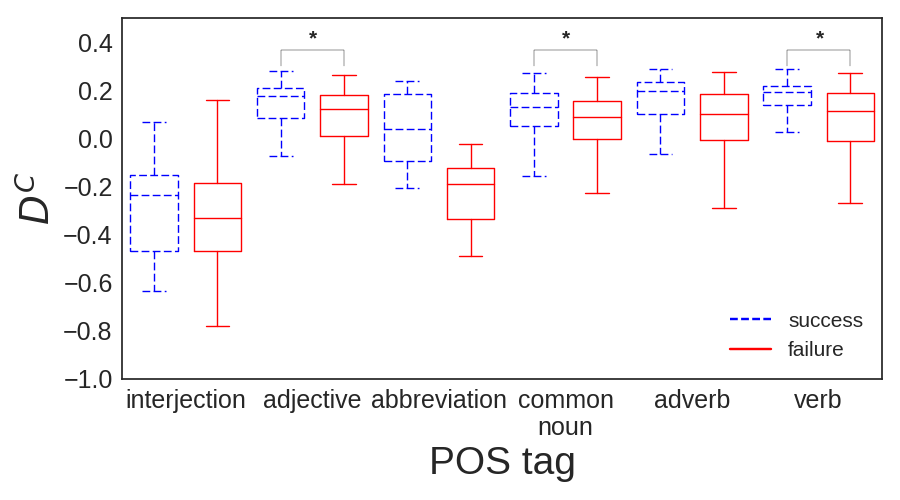
\includegraphics[width=\columnwidth]{figures/success_vs_failure_matched_pos_C3_distribution.png}
%\caption{Distribution of $D^{L}$ values across successful and failed innovation, grouped by part of speech tag. 
%* indicates $p<0.05$ in one-tailed t-test between successful and failed $D^{L}$ values.}
%\label{fig:success_vs_failure_pos_C3_distribution}
%\end{figure}
%
%\paragraph{Robustness checks}
%We perform this same classification task for a range of history lengths, $k \in \{2 ... 8\}$, and find similar accuracy results across the feature sets: \model{f+L+S} outperforms \model{f+L} and \model{f+S}, which outperform \model{f}.
%%(maximum $\model{f}$ accuracy 54.15\%, minimum $\model{f+L}$ accuracy 56.97\%, minimum $\mathtt{f+S}$ accuracy 56.26\%). \ian{confirmed with both all-value prediction and mean-value prediction}.
%Next, based on the distribution of context dissemination across part of speech groups (see \autoref{fig:pos-cd-dist}), it may seem that context dissemination serves as a proxy for differentiation by part of speech.
%%\ian{need to check $D^{L}$ coefficient in \model{f+L+S+P}}.
%To address this concern, we included part-of-speech tags as predictors in the full model in place of context dissemination (\model{f+S+P}) in the prediction task outlined above and found that the model yielded a lower mean accuracy (64.0\%) than the model with the rest of the predictors (\model{f+L+S}) ($t=-29.6, p < 0.0001$). 
%%\ian{also found that $D^{L}$ coefficient in $f+L+S+P$ model was similar to $f+L+S$ model: $\beta_{D^{L}} = 3.66$}
%%To address this concern, we included part-of-speech tags as predictors in the binary classification task and found that their inclusion in the full model resulted in lower prediction accuracy (comparing \model{f+L+S} versus \model{f+L+S+P}, $t=8.79, p < 0.0001$). 
%% output/pos_vs_regular_accuracy_t_test_results.tsv
%We further test this hypothesis by grouping the successful and failed innovations by part of speech tag and comparing the mean context dissemination of success versus failure words, plotted in \autoref{fig:success_vs_failure_pos_C3_distribution}.
%Across the most frequent speech groups (verbs, common nouns and adjectives), failed innovations have significantly lower context diversity than successful innovations in the same category.
